\subsection{Binary Star Evolution}\label{sec:BinaryStarEvolution}

\subsubsection{Class Hierarchy}\label{sec:BSEClassHierarchy}

The BSE inheritance hierarchy is as follows:

BinaryStar\ \rarr\ BaseBinaryStar

\tabto{2em}(Star\ \rarr\ )\tabto{7em}BinaryConstituentStar (star1) \\
\tabto{2em}(Star\ \rarr\ )\tabto{7em}BinaryConstituentStar (star2)

The main class for binary star evolution is the \textbf{BinaryStar} class.  The BinaryStar class is a wrapper that abstracts away the details of the binary star and the evolution. Internally the BinaryStar class maintains a pointer to an object representing the binary star being evolved, with that object being an instance of the \textbf{BaseBinaryStar} class.

The \textbf{BaseBinaryStar} class is a container class for the objects that represent the component stars of a binary system. An instance of the BaseBinaryStar class is a binary system being evolved by COMPAS, and contains a \textbf{BinaryConstituentStar} class object for each of the component stars (i.e. the primary and secondary stars), as well as data structures and algorithms specific to the evolution of a binary system.

The \textbf{BinaryConstituentStar} class is a wrapper class for the SSE Star class. An instance of the BinaryConstituentStar class is a single component star of a binary system being evolved by COMPAS, and contains a Star class object that will evolve over time through various SSE classes shown in Figure~\ref{fig:SSE_ClassDiagram}. The BinaryConstituentStar class defines additional data structures and algorithms (to the data structures and algorithms provided by the SSE classes) required to support the evolution of a binary system component star.

The BaseBinaryStar class is the main class for the underlying binary star object held by the BinaryStar class.  The BaseBinaryStar class defines all member variables that pertain specifically to a binary star, and many member functions that provide binary-star specific functionality.  Internally, the BaseBinaryStar class maintains pointers to the two \textbf{BinaryConstituentStar} class objects that constitute the binary star.

The BinaryConstituentStar class inherits from the Star class, so objects instantiated from the BinaryConstituentStar class inherit the characteristics of the Star class, particularly the stellar evolution model.  The BinaryConstituentStar class defines member variables and functions that pertain specifically to a constituent star of a binary system but that do not (generally) pertain to single stars that are not part of a binary system (there are some functions that are defined in the BaseStar class and its derived classes that deal with binary star attributes and behaviour -- in some cases the stellar attributes that are required to make these calculations reside in the BaseStar class so it is easier and cleaner to define the functions there).


\newpage
\subsubsection{Evolution Model}\label{sec:BSE_EvolutionModel} 

The high-level binary evolution model is shown in Figure~\ref{fig:BSE_FlowChart}.

The binary evolution model is driven by the \textbf{Evolve()} function in the BaseBinaryStar class, which evolves the star through its entire lifetime by doing the following:

\bigskip
if touching \\
\tabto{3em} STOP = true \\
else \\
\tabto{3em}calculate initial time step \\
\tabto{3em}STOP = false

\medskip
DO WHILE NOT STOP AND NOT max iterations:

\tabto{3em}evolve a single time step \\
\tabto{5em}evolve each constituent star a single time step (see SSE evolution)

\tabto{3em}if error OR unbound OR touching OR Massless Remnant \\
\tabto{5em}STOP = true \\
\tabto{3em}else \\
\tabto{5em}evaluate the binary

\tabto{7em}calculate mass transfer \\
\tabto{7em}calculate winds mass loss

\tabto{7em}if common envelope \\
\tabto{9em}resolve common envelope \\
\tabto{7em}else if supernova \\
\tabto{9em}resolve supernova \\
\tabto{7em}else \\
\tabto{9em}resolve mass changes

\tabto{7em}evaluate supernovae

\tabto{7em}calculate total energy and angular momentum \\
\tabto{7em}update magnetic field and spin: both constituent stars

\medskip
\tabto{5em}if unbound OR touching OR merger \\
\tabto{7em}STOP = true \\
\tabto{5em}else \\
\tabto{7em}if NS+BH \\
\tabto{9em}resolve coalescence

\tabto{9em}STOP = true \\
\tabto{7em}else \\
\tabto{9em}if WD+WD OR max time \\
\tabto{11em}STOP = true \\
\tabto{9em}else \\
\tabto{11em}if NOT max iterations \\
\tabto{13em}calculate new time step

\begin{figure}
    \begin{center}
	    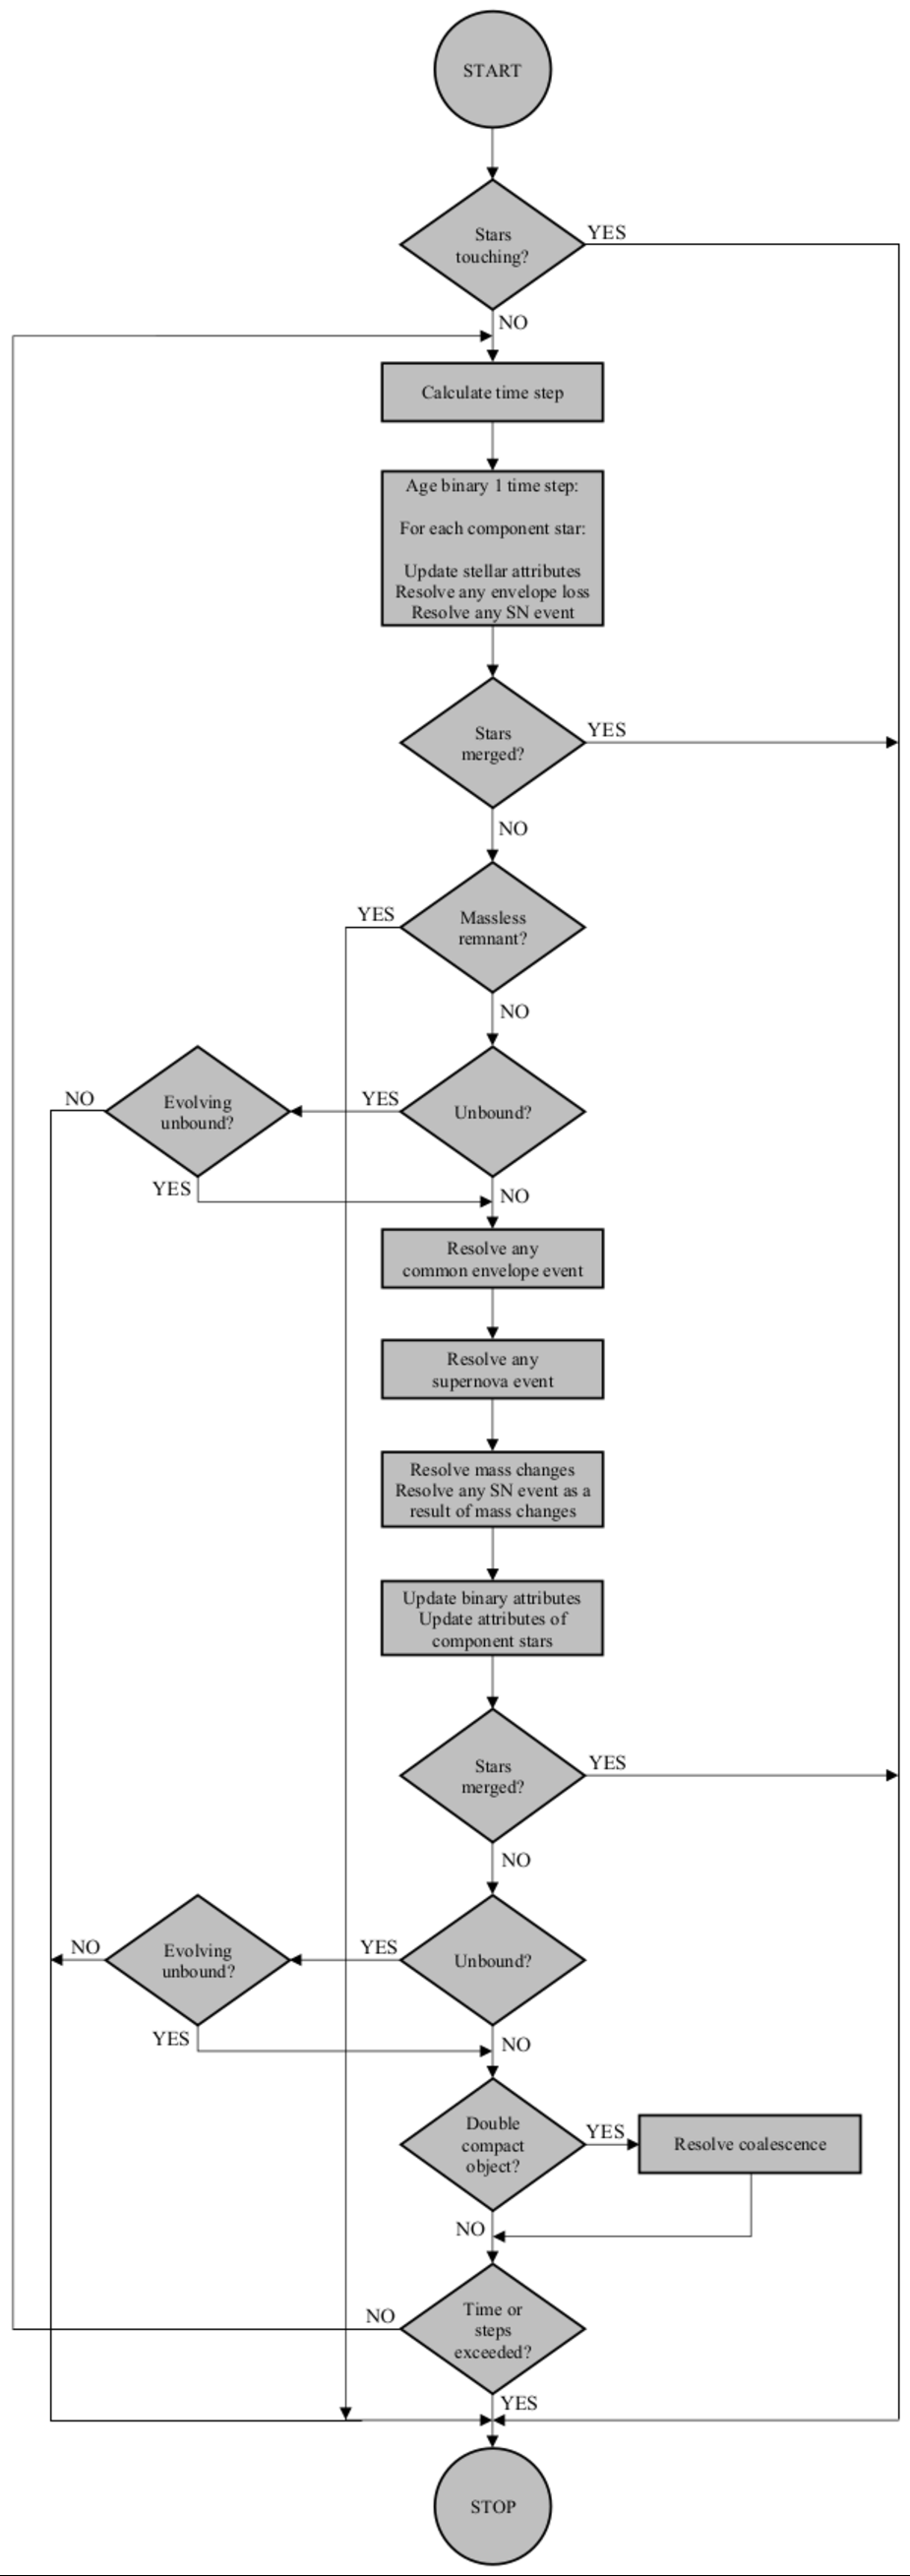
\includegraphics[viewport = 0 0 440 1252, width = 7.75cm, clip]{sections/images/BSE_FlowChart.pdf}
    \end{center}
    \vspace{-8.00mm}
    \caption{High-level BSE evolution.}
    \label{fig:BSE_FlowChart}
\end{figure}
